% !TEX program lualatex
\documentclass{EU-report}
\usepackage{longtable}
\usepackage[style=verbose-trad1,bibstyle=eubibstyle,sorting=none,maxbibnames=100,firstinits=true,backend=bibtex]{biblatex}

\bibliography{references-Groningen,utz-collection,science-tlp}

\graphicspath{{./}{./Figures/}{../Figures/}}

\begin{document}

\begin{center}
\vfill
Project Number: 737043\\[1cm]
Project Acronym: \textbf{TISuMR}\\[1cm]
Project Title: \textbf{Integrated Tissue Slice Culture and NMR Metabolomics
  --- A Novel Approach Towards Systemic Understanding of Liver Function And Disease}\\
\vfill
{\Huge TISuMR Device Specification\\}
\vfill
\includegraphics[width=5cm]{tisumr-logo}
\end{center}
\vfill
Document version: 0.0.0 \\
Last modified: \today
\vspace{1cm}

\clearpage
\section{Executive Summary}

\section{Change History}
\begin{center}
	\begin{tabular}{lrp{7cm}r} \hline\hline
		\emph{Version} & \emph{Mod. Date} & \emph{Summary of changes} & \emph{Author} \\
		\hline
		0.0.0 & 22/5/2019 & Initial discussion version & ms, mu\\
		\hline\hline
	\end{tabular}
\end{center}
\clearpage

% ========== Edit your name here
%\author{}
%\title{TISuMR device specifications}
%\maketitle

%\medskip
\section{Scope of this document}
TISuMR is a collaboration project between University of Southampton, University
of Groningen and Karlsruhe Institute of Technology. The aim of the project is to
develop technologies for NMR (nuclear magnetic resonance) compatible
microfluidic perfusion culture of PCLS (precision cut liver slices).
The devices that are being developed at the three project partner sites
are built for different aims (high-resolution liquid NMR spectroscopy of the
perfusion fluid, high-resolution magic-angle spinning NMR spectroscopy,
or conventional analysis using HPLC and other techniques). These different
approaches lead to different interfacing requirements for the perfusion system.
In order to ensure comparability of the results, it is necessary to standardise
certain aspects of the design. This will ensure identical culture conditions,
as well as a common standard to judge the performance of the culture
system and basic viability of the tissue slices.

This document defines the specifications for a device design to be qualified as
a TISuMR device. All the TISuMR personnel will follow these requirements for
device design if the device is used for TISuMR research. Possible variations are
also given to cater to specific experimental needs.

Changes to this document will be decided in the TISuMR meetings. The intended
changes will be communicated to all the partners before the meeting to think
upon. All the partners should agree for a change to be made final. This document
will be available on
\url{https://github.com/marcel-utz/tisumr-device} to obtain the latest version
of the document. Marcel Utz will own the master copy and will be responsible to
implement the changes. A drawing of the proposed device is shown in
Fig.\ref{fig:tisumr-device}

\section{Required Specifications}
\begin{itemize}
\item \textbf{Culture chamber geometry:} The culture chamber is cylindrical in
shape with a diameter of 7$\pm$1 mm and a depth of 500$\pm$100 $\mu$m.
%The overall thickness of the device is less than 1 mm.
% mu: I suggest removing this, as it is not essential.
\item \textbf{Perfusion geometry:} The perfusion fluid flows around the PCLS.
There can be more than one inlets and outlets. The inlet and outlet channels
have cross sectional dimensions of 200$\pm$100$\times$200$\pm$100 $\mu$m$^2$.
\item \textbf{Chip or device material:} Polycarbonate is used for the chip or
device fabrication.
\item \textbf{Temperature:}. The PCLS culture is performed at
37$\pm$0.5$^{\circ}$.
\item \textbf{Gas composition:} Either carbogen (95 \% O$_2$ + 5 \% carbon
dioxide) or a mixture (80 \% O$_2$+ 10 \% nitrogen +5 \% carbon dioxide) is used
for the culture.
\item \textbf{Viability standards:} Adenosine tri(phosphate) (ATP) content in
the tissue slice after culture is used as a measure of viability. As a rule,
tissue slices can be considered viable if they contain at least 6~pmol of ATP
per mg of protein. {\color{red}The protocols for ATP determination are given in section ...}
\item \textbf{Medium composition:} William E  with Glutamax + Glucose (1.375
g/500mL William E medium) + Gentamycine (500$\mu$L/500mL)
\item \textbf{Sterilization:} Ethanol will be used for sterilization.
{\color{red} Provide ethanol concentration and minimum exposure time.
Define internal vs external sterilisation. How are ancillary perfusion
equipment to be sterilised (e.g., tubing, syringes, connectors, gaskets?)}
\end{itemize}

\section{Allowed variations}
\begin{itemize}
\item \textbf{Detailed fluidic paths:} Fluidic network can be designed freely.
\item \textbf{Flow protocol:} The media can be flowed by different types of
pumps or centrifuge.
\item \textbf{Fabrication method:} The devices can be made through machining or
bonding layers by different protocols.
\item \textbf{Flow rates:}. Range of flow rates will be decided through
optimization.
\end{itemize}

\begin{figure}
\centering

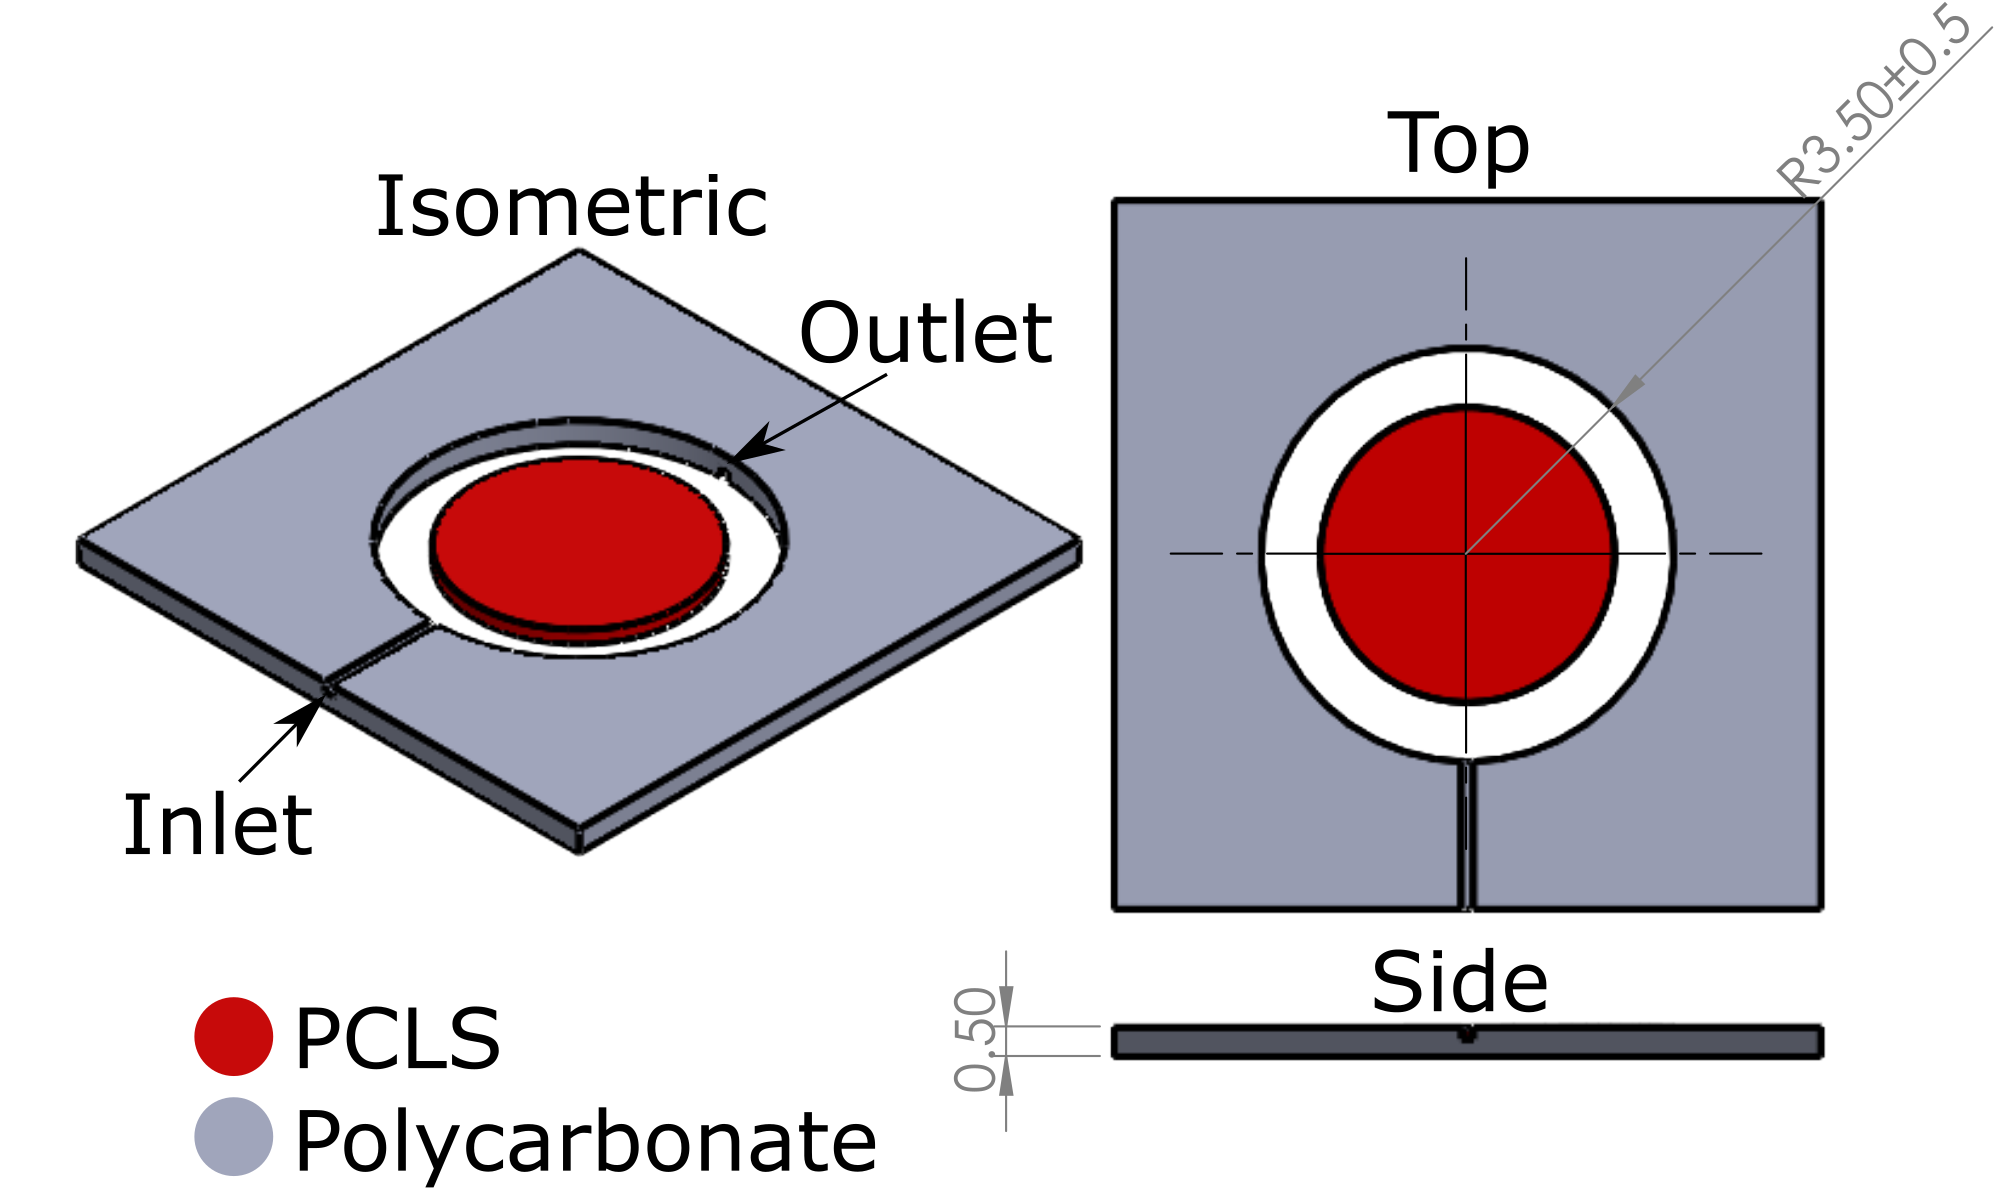
\includegraphics[width=.8\linewidth,keepaspectratio=true]{./device/tisumr-device.png}
\caption{Isometric, top and side views of the device. The diameter of the PCLS
chamber is 0.7 mm. The thickness of the chamber is 0.5 mm.}
\label{fig:tisumr-device}
\end{figure}

\end{document}
